\chapter{Finite Mean Flow Simulations}
\label{app_mean_flow}

In the main text, I focused on one particular LAPD experiment, which contained little mean ${\bf E \times B}$ flow and flow shear. Focusing on this null flow experiment
allowed me to model the system with a smaller number of linear terms in the equation set than if the experiment had contained significant ${\bf E \times B}$ flow. 
Furthermore, neglecting mean flow and flow shear eliminated linear instabilities such as Kelvin-Helmholtz
and Rotational Interchange, which are both flute-like ($k_{\para} = 0$). With these present, it can be difficult to differentiate between the nonlinear instability and these linear instabilities,
though careful energetics analysis can do so.
Furthermore, the low flow experiments have proven to be easier to successfully simulate than
the high flow experiments, and the null flow experiment and simulations contain so much interesting physics that they deserve study in their own right.

In this appendix, I review preliminary results of simulations and analysis of finite mean flow experiments recently performed in LAPD. 
I choose to present this in an appendix rather because it is preliminary, highly unpolished work. 
Moreover, mean flow shear suppression is somewhat off topic and wouldn't necessarily add to the main points that I developed in the main text. 
But I cannot emphasize enough how important well-validated, well-analyzed mean flow simulations would be
to the understanding of these experiments and the important effects that they were designed to illuminate. Because of that, I present here my preliminary results of some mean flow simulations
so that others can build upon this work.


\section{The LAPD Biasing Experiment}
\label{s_biasing_exp}

\begin{figure}
\centerline{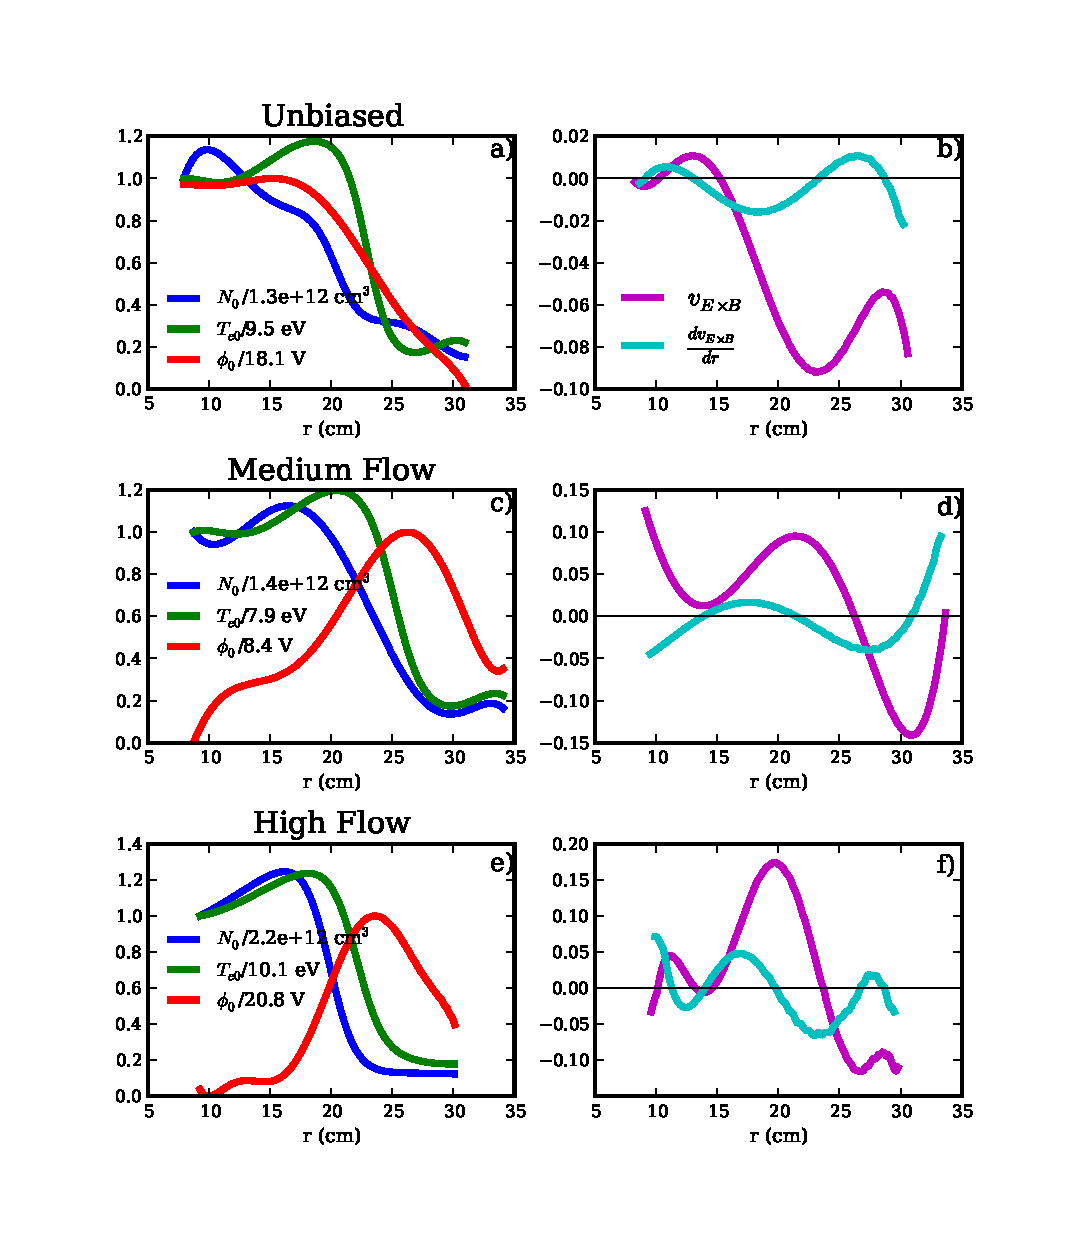
\includegraphics[]{flow_profiles}}
\caption{Equilibrium profiles for different biases}
\label{flow_profiles}
\end{figure}

The high ${\bf E \times B}$ flow and flow shear LAPD experiments are relevant to tokamak research, specifically research into the High Confinement Mode (H-mode)
and the transition to the H-mode. Researchers have long realized that H-mode is associated with strong toroidal rotation of the tokamak plasma and that the shear associated with this rotation
is the likely cause of the decrease in energy transport. The particular physical mechanism of turbulent-shear interaction that causes the flux suppression is still an area of intense research.

To investigate the interaction between flow and turbulence, David Schaffner, Troy Carter, and others recently set up an experiment on LAPD
in which they varied the mean flow and flow shear. In order to vary the ${\bf E \times B}$ flow, they inserted a biasable azimuthal limiter into LAPD. The limiter has radius ~26 cm, and
can be biased with respect to the cathode. When the cathode and limiter are unbiased -- maintained at the same potential -- no net current flows between them, and they act
as a single conducting plate. In this case, my discussion of the sheath in Sec.~\ref{ss_bs_bc}, accounts for how the plasma potential is set by
the current into the plate and the temperature profile. I considered the case for a floating conducting plate, in which, $\phi = \Lambda T_e /e$, with 
$\Lambda = \rm{ln} \left( \frac{1}{2 \sqrt{\pi}} \sqrt{\fmie}  \right)$, where $\phi$ is the potential difference between the sheath edge and the conducting plate. If the plate is not
floating, but drawing a current, as is the case with the cathode, the proportionality factor relating $\phi$ and $T_e$ is different and not necessarily constant:
\beq
\label{lambda_r}
\Lambda(r) = {\rm{ln}} \left( \frac{1}{2 \sqrt{\pi}} \sqrt{\fmie} \frac{1}{1 - \frac{J_\para}{e n c_s}} \right).
\eeq
Nevertheless, the radial shape of $\phi$ somewhat mimics that of $T_e$ so long as there is no potential difference between the limiter and cathode. 
I show the equilibrium density, electron temperature, and potential profiles
for the case of the unbiased limiter in Fig.~\ref{flow_profiles} a). The potential profile -- to which I have added an arbitrary constant -- has the same general shape as the temperature profile,
but is somewhat different due to the radial dependence of $\Lambda$ in Eq.~\ref{lambda_r} on the non-uniform cathode current.
Moreover, in Fig.~\ref{flow_profiles} b), I plot the azimuthal $v_{E \times B}$ and its radial derivative, the shear. Both are normalized by the same potential as $\phi_0$.

When the cathode and limiter are biased -- maintained at a different potential -- they draw different currents. 
Then the proportionality function $\Lambda(r)$ becomes a strong function of radius, and $\phi$ no longer mimics $T_e$. 
I show the equilibrium profiles when relatively
high biasing is applied in Fig.~\ref{flow_profiles} c), and when very high biasing is applied in Fig.~\ref{flow_profiles} e). Notice that the direction of the radial electric field -- equivalent
to $v_{E \times B}$ -- changes inside of the limiter radius due to the biasing. Also note that although I do not show it in Fig.~\ref{flow_profiles}, there is a level of intermediate
biasing in which the radial electric field inside of the limiter radius nulls out. I based my simulations and analysis in the main text off of this configuration.

Another way to see why the radial electric field changes when the cathode and limiter are biased is to picture the system as a circuit. The circuit runs from the limiter
through the biasing source -- maintaining a potential difference -- through the cathode and finally through the plasma itself, which fills the region between the cathode and the limiter.
The electrons in the plasma can carry the current along the magnetic field lines, but many of the field lines that terminate on the cathode are radially separated from the limiter field lines,
so a radial current forms to complete the circuit. This radial current is primarily carried by ions. Recall from Sec.~\ref{s_vorticity_eqn} that there are two contributions from the ions
to the cross-field current: the polarization current and the Pederson current. The polarization current due to the ions, however, is
\beq
\label{pol_curr}
J_{pi} \approx e n \vec{b} \times \left( \pdt + {\bf v}_E \cdot \grad \right) {\bf v}_E.
\eeq
The time derivative term cannot contribute to the equilibrium current. Then, the radial part of the equilibrium polarization current is only
\beq
\label{rad_pol_curr}
J_{pir} \approx \frac{e n }{r} E_\theta \pdiff{E_\theta}{\theta}.
\eeq
But there is no equilibrium $E_\theta$, so $J_{pir} \approx 0$. It's likely that other terms that can contribute to the polarization current that I ordered out in Sec.~\ref{s_vorticity_eqn}
could produce a radial polarization current, but I do not try to derive them here. Rather, I attribute all of the equilibrium radial current to the Pederson current, which
is driven by a time-independent radial electric field. The radial electric field, therefore, is
necessary to complete the circuit. Biasing then, through sheath properties and plasma currents, can change the radial potential profile.
This, of course, produces mean azimuthal ${\bf E \times B}$ flows that can have radial shear.

In the biasing experiments documented in Schaffner et al.~\cite{schaffner2012,schaffner2013}, the bias voltage is changed incrementally through about $30$ different values. 
The mean flow of the unbiased state points in the ion diamagnetic direction. As the bias increases, this flow nulls out and then changes direction inside of the limiter radius, which is
clear from the few profiles I show in Fig.~\ref{flow_profiles}. Moreover, the radial flow shear also changes with changing bias, with the shear rate $\gamma_s$ ranging from zero to about five times
the autocorrelation time $\tau$. Their analysis shows that the radial particle flux and the density scale length are inversely proportional to the 
flow shear regardless of the flow direction~\cite{schaffner2012}. 
The experiments clearly show that flow shear suppresses radial particle flux through suppression of turbulent density fluctuations. 
The mechanism that causes this, however, is less obvious, and they try to answer this by comparing shear scaling properties to various theoretical predictions~\cite{schaffner2013}.
Simulations with highly resolved spatial features can help this effort.

Other interesting findings in the biasing experiment include a change in the shape of the frequency spectra with biasing. As the flow and flow shear become large, a coherent feature,
seen as a sharp peak at the low end of the frequency spectra, emerges. Furthermore, the spectra become more exponential at high frequency as the flow and flow shear increase. These signal
possible changes in the nature of the turbulence. The coherent feature, for instance, indicates the presence of a coherent mode, possibly due to a flow instability. The exponential spectra
might indicate a change in the chaotic properties of the turbulence, namely, a decrease in the attractor dimension. This speculation can likely be sorted out with
the help of well-validated numerical simulations. Therefore, I have attempted to simulate a few of the different biased cases and analyze the results using the tools I used in the main
text on the null flow experiment and simulations.


\section{Simulation Model}
\label{s_sim_model}

The simulation model that I use is the same that I use in the main text (See Chapter~\ref{c_braginskii}) with mostly obvious and straight forward additions to account for the mean potential
profiles in the experiments that I simulate in this appendix. I treat the potential the same way that I treated the density and temperature in the main text -- by dividing it into a time-independent
equilibrium part and a time-dependent fluctuating part. With this, the model equations become:
\beqar
\label{ni_eq_flow}
\pdt N = - {\mathbf v_E} \cdot \grad N_0 - {\mathbf v_{E0}} \cdot \grad N - N_0 \gradpar \vpe + \mu_N \gradperp^2 N + S_N + \{\phi,N\}, \\
\label{ve_eq_flow}
\pdt \vpe = - {\mathbf v_{E0}} \cdot \grad \vpe - \fmie \frac{T_{e0}}{N_0} \gradpar N \nonumber \\
- 1.71 \fmie \gradpar T_e + \fmie \gradpar \phi - \nue \vpe + \{\phi,\vpe \}, \\
\label{rho_eq_flow}
\pdt \varpi = - {\mathbf v_E} \cdot \grad \varpi_0 - {\mathbf v_{E0}} \cdot \grad \varpi- 
\frac{1}{r} \pdiff{\phi_0}{r} \left(\pdiff{N_0}{r} \pdiffxy{\phi}{r}{\theta} - \pdiffs{\phi_0}{r} \pdiff{N}{\theta} \right) \nonumber \\
 - N_0 \gradpar \vpe  - \nuin \varpi + \mu_\phi \gradperp^2 \varpi + S_\phi + \{\phi,\varpi \}, \\
\label{te_eq_flow}
\pdt T_e = - {\mathbf v_E} \cdot \grad T_{e0} - {\mathbf v_{E0}} \cdot \grad T_e - 1.71 \frac{2}{3} T_{e0} \gradpar \vpe + \frac{2}{3 N_0} \kpe \gradpar^2 T_e  \nonumber \\
- \frac{2 m_e}{m_i} \nue T_e  + \mu_T \gradperp^2 T_e +  S_T + \{\phi,T_e\}.
\eeqar

I simulate three different biasing experiments -- those corresponding to the profiles that I showed in Fig.~\ref{flow_profiles}. I use a potential source $S_\phi$ in the same way that I
use density and temperature sources (see Sec.~\ref{ss_sources}). However, while it is clear that the turbulent flux will cause the total radial density and temperature profiles
-- equilibrium plus flux-surface averaged fluctuating component -- to relax over time, it is not obvious what affect if any the turbulence should have on the total potential profile. 
The reason is that the turbulent Reynolds Stress, which comes from the flux-surface average of the $\{\phi,\varpi \}$ term in Eq.~\ref{rho_eq_flow} 
can drive time-dependent zonal flows and time-independent mean flows -- the Reynolds Stress is a three-wave transfer in the terminology of the energy dynamics. Generally, however,
radially non-oscillatory mean flows require an external torque due to angular momentum conservation.

When I simulated the null flow experiment and even the unbiased experiment without a potential source, no noticeable mean flow developed. 
However, when I simulated the medium flow and high flow experiments, a mean
flow did form, presumably because my radial boundary conditions apply a significant torque to the plasma. In any case, this means that I do have to use a potential source to maintain
the physically relevant total potential profile. In most cases it would probably be best to use a fixed potential source because the source that I use (see Sec.~\ref{ss_sources})
largely removes the zonal flows as well as the mean flows. I don't think the zonal flows are that important, as I showed in Fig.~\ref{zf_gamma_spec}, but they might be in the higher flow
cases.

Additionally, I use periodic axial boundary conditions for these simulations because the boundary conditions didn't seem to have much affect on the turbulence in the null flow simulations.
As for the artificial diffusion and viscosity levels -- which I use as a free parameter to match the level of turbulence between the simulations and experiment -- I use values of
$1.2 \times 10^{-3}$, $2 \times 10^{-3}$, and $0$ for the unbiased, medium flow, and high flow simulations respectively. Also, as I discussed in Appendix~\ref{app_bout}, I use a first order
upwind advection scheme for the advective nonlinearities in these equations, which introduces a lot of numerical diffusion.


\section{New Linear Instabilities}
\label{s_flow_inst}

The addition of an equilibrium potential profile introduces two new linear instabilities into the picture. First, the Kelvin-Helmholtz (KH) instability, which is a fluid instability -- as opposed to
a plasma-specific instability -- is caused by the radial gradient in the azimuthal ${\bf E_0 \times B}$ velocity. Second is the rotational interchange instability (RIC), which is caused by the bulk
rotation of the plasma in the presence of the magnetic field.

The KH instability is a convective vorticity instability, meaning it can be described by the simple equation
\beq
\label{kh_inst_eq}
\pdiff{\varpi}{t} = - {\bf v} \cdot \grad \varpi.
\eeq
The instability occurs when there is a shear in the velocity gradient. Diagrams of the mechanism can be found in Manneville p. 227~\cite{manneville2004}, Drazin and Reid p.15~\cite{drazin1981},
and in other hydrodynamic instability books. Their treatments all follow Batchelor's~\cite{batchelor1967}. I summarize the mechanism as follows.
Imagine a boundary layer separating two flows that have equal speeds but velocities going in different directions. Since
the vorticity is just the curl of the velocity, this boundary layer is a vortex sheet. Now a sinusoidal vorticity perturbation on this sheet causes a sinusoidal ripple in the elevation
of the sheet. This ripple brings parts of the sheet into regions where the background flow is positive and other parts of the sheet into regions where the flow is negative. The vorticity on
the sheet is then advected by this background flow in such a way that it reinforces the initial sinusoidal vorticity perturbation, thus causing instability. This instability is 2D and requires
only a velocity gradient.
In the LAPD plasma, the mean flow is in the azimuthal direction and its gradient is in the radial direction. Since the instability is 2D, it need not have a finite wavelength in the axial direction,
potentially making it a flute mode. In Eq.~\ref{rho_eq_flow}, the terms that cause the KH instability are 
$- {\mathbf v_E} \cdot \grad \varpi_0$ and $- {\mathbf v_{E0}} \cdot \grad \varpi$.

The RIC instability is analogous to the more commonly known interchange instability in magnetic confinement devices like tokamaks. That interchange instability is a result of a curved magnetic
field that causes particles to feel a centrifugal force as they travel along the field. The RIC instability in LAPD is not caused by magnetic field curvature (there is none), but by the
centrifugal force on particles as they are rotated around the cylinder by the azimuthal mean flow. 
The force on the particles is ${\bf F} = m v_\theta^2/r \ \hat{{\bf r}}$. Forces on particles in magnetic fields cause drifts:
\beq
\label{force_drift}
v_d = \frac{1}{q} \frac{{\bf F \times B}}{B^2}.
\eeq
Since the centrifugal force due to rotation is independent of charge, the electron and ion fluids drift in different azimuthal directions. If there is a density perturbation, this drift will cause
a spatial charge separation, which causes azimuthal electric fields and thus, radial ${\bf E \times B}$ velocities. 
These radial velocities advect fluid of different density into this charge-separated region in such a way to enhance the original density perturbation. In this instability, unlike the drift wave
instability, the density and potential perturbations are $90^o$ out of phase, meaning that the instability grows but does not propagate -- if the electrons are adiabatic. In other words,
this instability does not require the adiabatic response, and it is 2D, so it can have infinite axial wavelength. And unlike in the KH instability, the density is not a passive scalar in the
RIC instability. The new term in Eq.~\ref{rho_eq_flow} that is responsible
for the RIC instability is $-\frac{1}{r} \pdiff{\phi_0}{r} \left(\pdiff{N_0}{r} \pdiffxy{\phi}{r}{\theta} - \pdiffs{\phi_0}{r} \pdiff{N}{\theta} \right)$.

\begin{figure}
\centerline{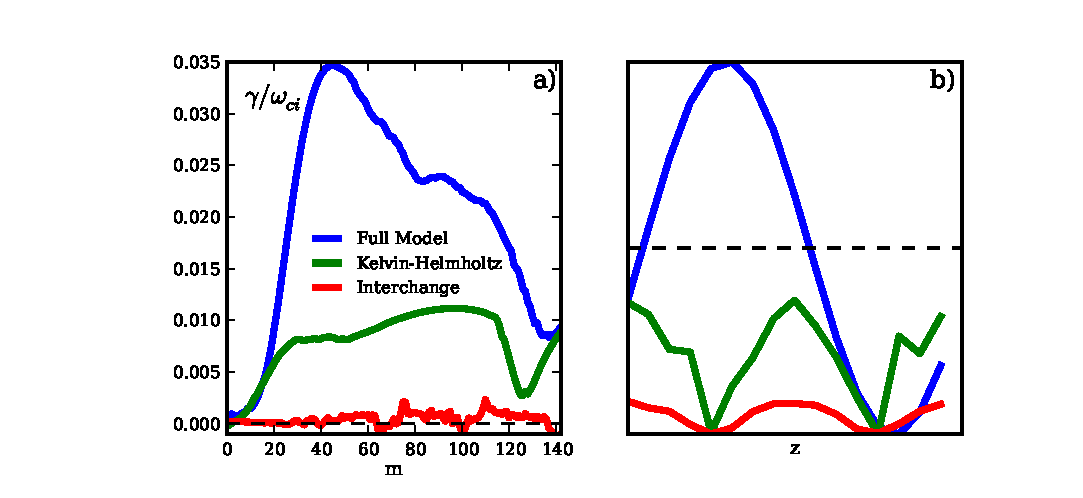
\includegraphics[]{flow_lin_inst}}
\caption{Linear growth rates and axial structures for high mean flow}
\label{flow_lin_inst}
\end{figure}

I show the growth rates as a function of $m$ number for the high flow simulation in Fig.~\ref{flow_lin_inst} a). The Full Model curve is the linear growth rate
for the full equation set. The growth rates are much higher than for the null flow case due primarily to the steep density and temperature gradients. For the Kelvin-Helmholtz and Interchange
curves, I have simulated only subsets of the equations. For both, I have removed the adiabatic response terms, which eliminate the drift wave drive. And for the KH simulation, I disregarded
the RIC term and vice versa for the IC simulation. From these results, it appears that the linear drift wave is most dominant with the KH instability also having significant positive growth
rate. The RIC instability is only marginally unstable. I note that the RIC and KH growth rate curves may be inaccurate, and that I need to confirm them with an independent calculation.
I also note that the growth rates might be very sensitive to the profiles, especially the potential profile, which I also must check.

In in Fig.~\ref{flow_lin_inst} b), I show the axial structure of the potential for the linear simulations that I used to calculate the growth rate. The Full Model curve has the shape of 
a single $n=1$ Fourier component, indicative of the linear drift wave that dominates the linear dynamics in this simulation. The KH and RIC axial structures
have large $n=0$ and $n=2$ Fourier components, and no significant $n=1$ Fourier component. The $n=2$ component is quite surprising and warrants further investigation.

\section{Statistical Comparisons to Experiment}
\label{s_flow_stats}

In Fig.~\ref{flow_statistics}, I compare a few statistical quantities of the density fluctuations -- $I_{sat}$ for the experiment --
between the flow experiments and the simulations corresponding to the profiles in Fig.~\ref{flow_profiles}. The top row
of plots -- a), b), and c) -- are based on the unbiased experiment and simulation, the middle row --  d), e), and f) -- derive from the medium flow experiment and simulation, 
while the bottom row -- g), h), and i) -- come from the high flow experiment and simulation. The first column plots -- a), d), and g) -- 
show the frequency power spectrum, the middle column shows the probability distribution function of the fluctuations, while the last column displays the radial RMS values of the fluctuations.

\begin{figure}
\centerline{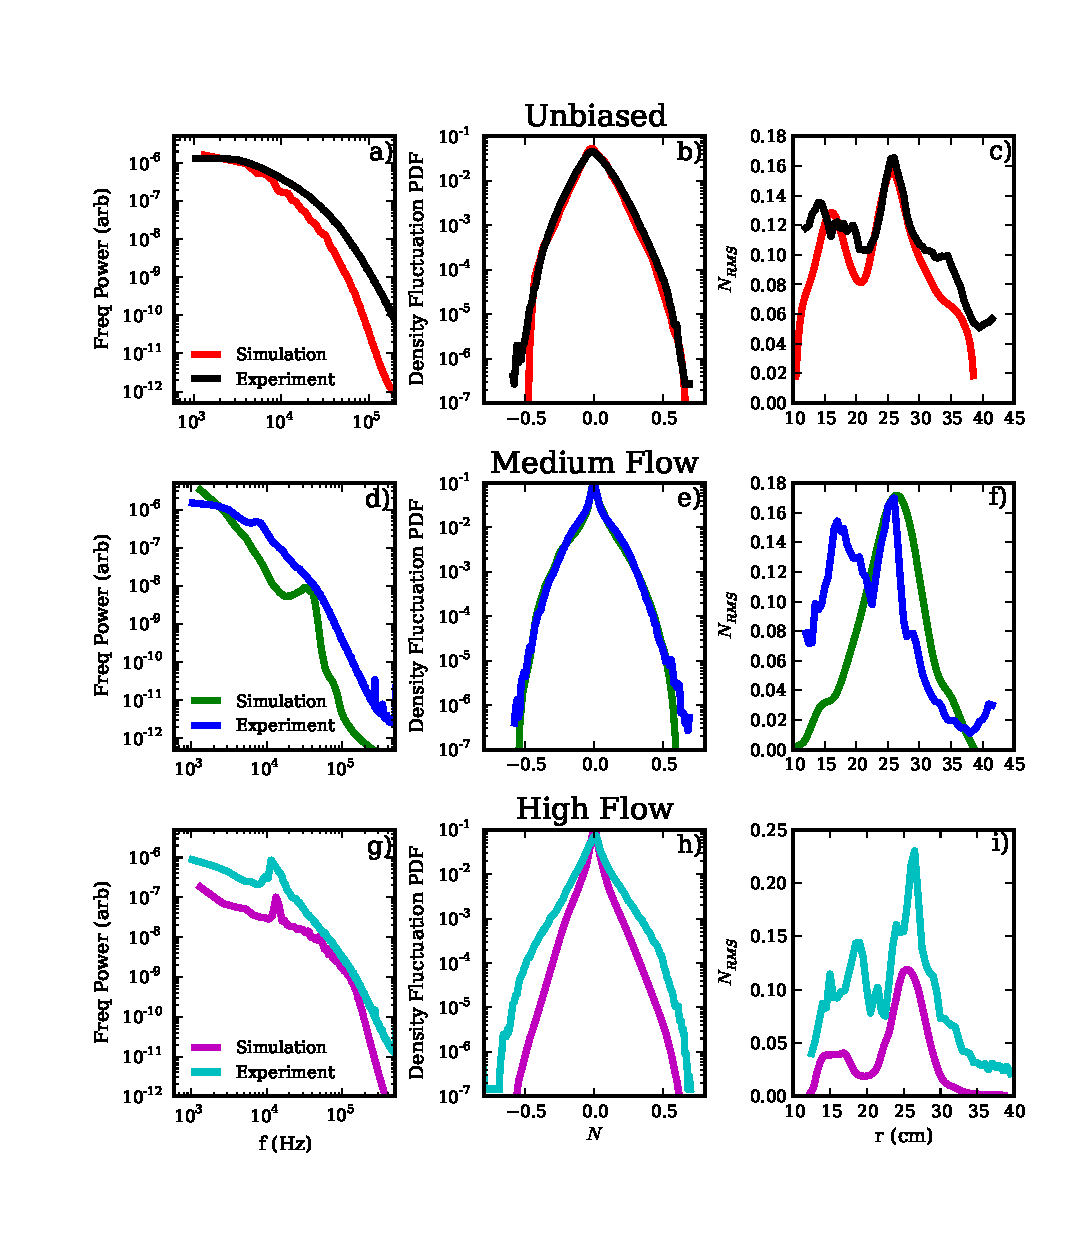
\includegraphics[]{flow_statistics}}
\caption{Mean flow experiment and simulation statistical comparisons}
\label{flow_statistics}
\end{figure}

For the unbiased case, the simulation matches the experiment quite well -- at about the same level as the null flow experiment and simulation in the main text. Moreover,
the statistical quantities for the unbiased simulation and experiment closely resemble those of the null flow experiment (see Fig.~\ref{n_statistics}) except for the fluctuation peak at $\sim 26$ cm
in the unbiased case, which isn't present in the null flow statistics.
The medium and high flow simulations, on the other hand, leave much to be desired with regards to their match against experiment. The medium flow simulation PDF matches the experimental PDF very well,
although I use my free parameter -- artificial diffusion and viscosity coefficient -- to match the standard deviation of the PDF of the simulation with the experiment. 
The skewness and kurtosis, however, are similar, and I do not control them.
Furthermore, the medium flow simulation and experiment both have a strong fluctuation level at $\sim 26$ cm, but the experiment has another peak at $\sim 16$ cm that the simulation does not.
Also, the simulation frequency spectra is qualitatively different than that of the experiment. 
The simulation frequency spectra has a strong coherent peak that is lacking in the experiment. I notice that this is
a common feature of the simulations when I use a high level of artificial diffusion. Presumably, then, this feature would disappear when I lower the diffusion. However, this would cause
a mismatch in the fluctuation level. I presume that I would be better served by lowering the diffusion and finding the cause of the then unphysically large fluctuation levels.
Obviously, the simulation model has some issue in this case. Perhaps my profiles have some unphysical feature in them, or maybe the zonal flows play a more
important role in saturating this case than in the unbiased case. This requires investigation.

For the high flow simulation, the qualitative match to the experiment is actually very good, including the match of the location of a coherent feature in the frequency spectrum at about $12$ kHz. 
However, the level of fluctuations is obviously too low in the simulation. Now I claimed that I use
the PDF standard deviation to set the free parameter, and in this instance, it appears that I should lower the free parameter to better match the fluctuation level. However, I have already
lowered the free parameter to \emph{zero} in this simulation, so I cannot lower it further. I note, though, that in addition to the artificial diffusion and viscosity that I put in these simulations,
there is also numerical diffusion and viscosity from the finite difference schemes, particularly from the first order upwind scheme that I use for the nonlinear advection terms in the flow
simulations. Therefore, the grid spacing that I use also acts like a tunable parameter for the diffusion and viscosity levels. In light of this, I have tried using finer grids, but I cannot
use too fine of grids because it increases simulation time, and more importantly, the very low level of diffusion leads to density positivity problems as I discuss in Appendix~\ref{app_bout}.
It appears then, that my partial linearization of the model equations, which is responsible for the lack of strict density and temperature positivity, may be an issue for this simulation.
But for now, I note that there is at least good qualitative agreement between this simulation and experiment. Nevertheless, due to my inability to fully validate the simulations, all conclusions
that I present are subject to change in the future.

\begin{figure}
\centerline{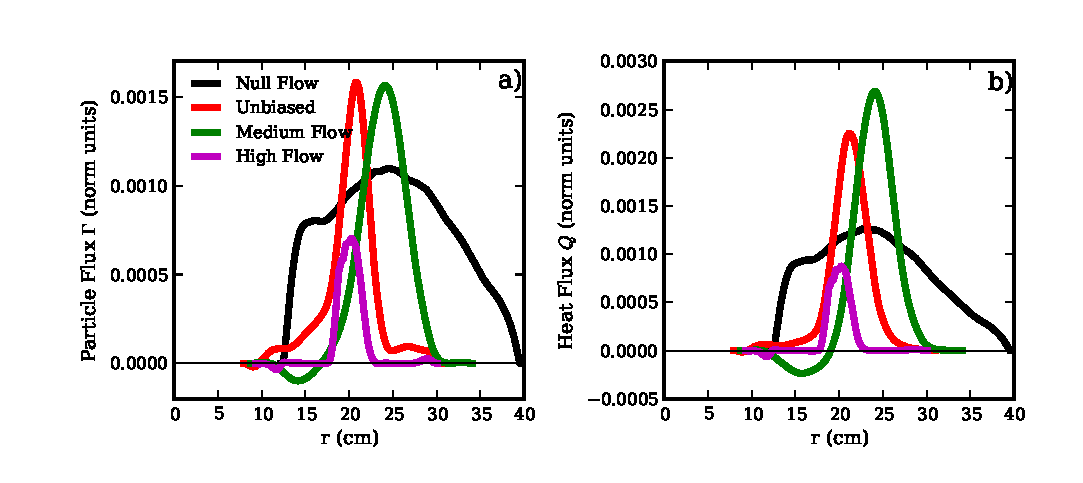
\includegraphics[]{flow_flux}}
\caption{Particle and heat flux for flow simulations}
\label{flow_flux}
\end{figure}

Next, in Fig.~\ref{flow_flux}, I display the particle flux $\Gamma = \left< N v_r \right>$ and heat flux $Q = \left< N T_e v_r \right> $. 
One of the first things one may notice in this figure is that the high flow simulation has much lower overall flux than the other simulations. 
This isn't a physical result because of the fluctuation level shortfall in the high flow simulation.
Additionally, the fluxes of the finite flow simulations are all much more peaked than they are in the null flow simulation. The peaks have radial locations similar to
where the flow profiles are peaked and where the shear profiles are at inflection points (see Fig.~\ref{flow_profiles}). For instance, the flux in the high flow simulation peaks at 20 cm.
From Fig.~\ref{flow_profiles} f), at 20 cm, the flow is at its largest absolute value, while the flow shear is about 0. Additionally, the width of the flux peak is on par with the width
of the shear inflection curve (from 17-23 cm). The same holds for the other two simulations, but to a lesser extent. These simulations seem to capture local shear suppression, although it's
not clear from this one figure if the flux is suppressed by the shear or if it is merely following the peaks in the density and/or temperature gradients. Simulations that evolve the equilibrium
gradients rather than taking them as input may be better suited to answering this question.

\section{Energy Dynamics Results}
\label{s_flow_en_dyn}

\subsection{The Broadband View}
\label{ss_broad_view}

The addition of the mean flow terms in Eqs.~\ref{ni_eq_flow}-\ref{te_eq_flow} -- those that contain ${\bf v}_{e0}$ or $\varpi_0$ -- only change the energy dynamics expressions slightly
from their form in Chapter~\ref{c_en_formalism}. In fact, only two terms -- both in Eq.~\ref{rho_eq_flow} -- actually
contribute to the energy dynamics: $- {\mathbf v_{E0}} \cdot \grad \varpi$ and 
$-\frac{1}{r} \pdiff{\phi_0}{r} \left(\pdiff{N_0}{r} \pdiffxy{\phi}{r}{\theta} - \pdiffs{\phi_0}{r} \pdiff{N}{\theta} \right) \nonumber$.
Mean flow advection terms such as $- {\mathbf v_{E0}} \cdot \grad N$ in Eq.~\ref{ni_eq_flow}, perhaps surprisingly, do not contribute to the energy dynamics. 
This can be seen by recalling the procedure for calculating the dynamics, which begins with multiplying Eq.~\ref{ni_eq_flow} by $T_{e0}/N_0 N$ and integrating over the volume. This term becomes
\beq
\label{en_mean_advec}
- \int_V \left( \frac{T_{e0}}{N_0} N {\mathbf v_{E0}} \cdot \grad N \right) dV = - \frac{1}{2} \int_r v_{E0} \frac{T_{e0}}{N_0} \int_{\theta,z} \pdiff{N^2}{\theta} r d\theta dz dr.
\eeq
Then, it is easy to see that the inner integral is zero due to the natural $\theta$ periodicity of $N$. The same holds for the mean flow advection terms in Eqs.~\ref{ve_eq_flow} and
~\ref{te_eq_flow}. The fluctuations are Doppler shifted by the mean flow, and even though the Doppler shift is a function of radius, the shift does not feed or dissipate the fluctuations
as a whole. This also holds true for each individual $(m,n)$ mode. 
These terms can, however, change the radial structures of the fluctuations, and this could be captured in different decompositions that do use radially decomposed modes,
but I don't focus on any of those here.

The linear mean flow advection of the vorticity ($- {\mathbf v_{E0}} \cdot \grad \varpi$) actually does provide a non-zero contribution to the energy dynamics because I obtain
the perpendicular kinetic energy by multiplying Eq.~\ref{rho_eq_flow} by $-\phi$ rather than by $\varpi$. In fact, this leads the $- {\mathbf v_{E}} \cdot \grad \varpi_0$ term in Eq.~\ref{rho_eq_flow}
to give zero energy contribution instead, for the same reason as the term in Eq.~\ref{en_mean_advec}.
Consequentially, only the $- {\mathbf v_{E0}} \cdot \grad \varpi$ and 
$-\frac{1}{r} \pdiff{\phi_0}{r} \left(\pdiff{N_0}{r} \pdiffxy{\phi}{r}{\theta} - \pdiffs{\phi_0}{r} \pdiff{N}{\theta} \right) \nonumber$ terms in Eq.~\ref{rho_eq_flow} contribute to the energy
dynamics that I formulated in Sec.~\ref{s_spec_en_dyn}. I identify the first of these terms as the contribution from the linear KH mechanism, and the second as the contribution from the
linear RIC mechanism. These are energy injection terms that take energy from the mean flow and deposit it into the perpendicular kinetic energy fluctuations ($\phi$ fluctuation energy).

\begin{figure}
\centerline{\includegraphics[]{flow_energy_spectra}}
\caption{Energy spectra for the high flow simulation}
\label{flow_energy_spectra}
\end{figure}

It should not be surprising that the addition of the mean flow does not change the nonlinear instability picture that I developed in Chapter~\ref{c_nlin_periodic}, especially for the unbiased
and medium flow cases. I do not show results from these two simulations here. Rather, I focus only on the high flow simulation energy dynamics since they are the most interesting,
and the others can simply be seen as intermediate cases of the null and high flow cases. First, I show the $(m,n)$ energy spectra for the high flow case in Fig.~\ref{flow_energy_spectra},
which can be compared to the null flow energy spectra in Fig.~\ref{energy_spectra}. Overall, the spectra of the two simulations are somewhat similar, but differences are visible.
The first clear difference is that the high flow simulation has a local energy peak at $|m|=1,|n|=2$ in all four fields, which is not present in the null flow case. 
Second, $E_N$ has more relative energy at $|n|=1$ for the high flow simulation, and this energy
is peaked at about $|m|=40$. The same is not true for $E_\phi$, where the null flow case seemingly has more relative energy at $|n|=1$, but the high flow case does have a local energy peak at
$|n|=0,|m|=40$. Clearly, the high flow case has more spectral features than the null flow case.

\begin{figure}
\centerline{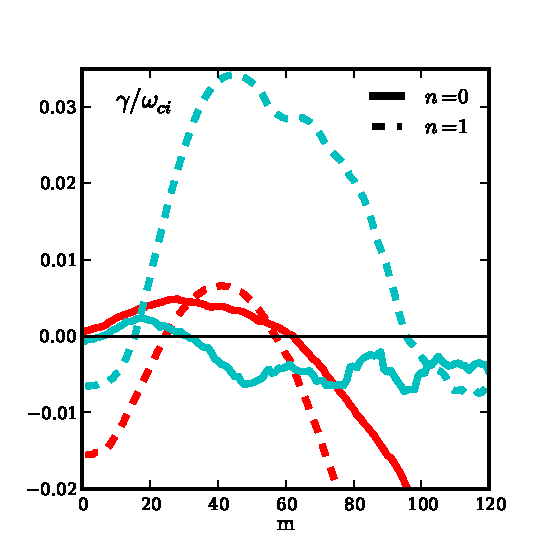
\includegraphics[]{flow_lin_vs_nl_gamma}}
\caption{High flow linear vs. nonlinear growth rates}
\label{flow_lin_vs_nl_gamma}
\end{figure}

To compactly describe some of the energy dynamics, I show the linear and nonlinear (turbulent) growth rates (explained in Sec.~\ref{ss_n0_supp}) in Fig.~\ref{flow_lin_vs_nl_gamma}. 
The red curves represent the nonlinear growth rates, while the cyan curves represent the linear growth rates. Note that I previously showed the linear growth rates of the different linear instabilities
in Fig.~\ref{flow_lin_inst}. Here, I am not breaking up the curves in terms of linear instabilities, but rather in terms of $n$ number. The $n=1$ curve, however, pretty closely
corresponds to the Full Model curve in Fig.~\ref{flow_lin_inst} a), but they are different because here, I have added a precise amount of artificial diffusion and viscosity in order to better compare to
the nonlinear growth rate curves, which have numerical diffusion and viscosity due to the finite difference advection scheme. That is the reason for the sharper falloff at high $m$ for the $n=1$
curve in Fig.~\ref{flow_lin_vs_nl_gamma} compared to the Full Model curve in Fig.~\ref{flow_lin_inst} a). Likewise, the $n=0$ curve here corresponds to the KH curve
in Fig.~\ref{flow_lin_inst} a), except here there is artificial viscosity.
Now like for the null flow case, for which I showed the linear and nonlinear growth rates in Fig.~\ref{lin_per_non0_gamma}, the high flow simulation nonlinear growth rates are 
much different from the high flow linear growth rates. This is a result of the same nonlinear instability mechanism that controlled the null flow case. Fig.~\ref{flow_lin_vs_nl_gamma}, by itself,
doesn't prove that the nonlinear instability mechanism is active because it is possible that the KH or RIC instabilities could be responsible for the positive $n=0$ growth rate. But a deeper look at
the energy dynamics reveals that this isn't the case, and that the nonlinear instability mechanism still dominates.
On the other hand, the high flow case does have a positive nonlinear growth rate for $n=1$, which is just as strong as the $n=0$ growth rate. Presumably, the linear drift wave instability is
so strong for this high flow case -- which has a high localized density gradient -- that it can compete with the nonlinear instability mechanism. Overall, despite the high mean flow,
the KH and RIC instabilities are not wholly significant, though they cannot be ruled out as factors for the coherent mode.

\subsection{The Coherent Mode}
\label{ss_coherent_mode}

\begin{figure}
\centerline{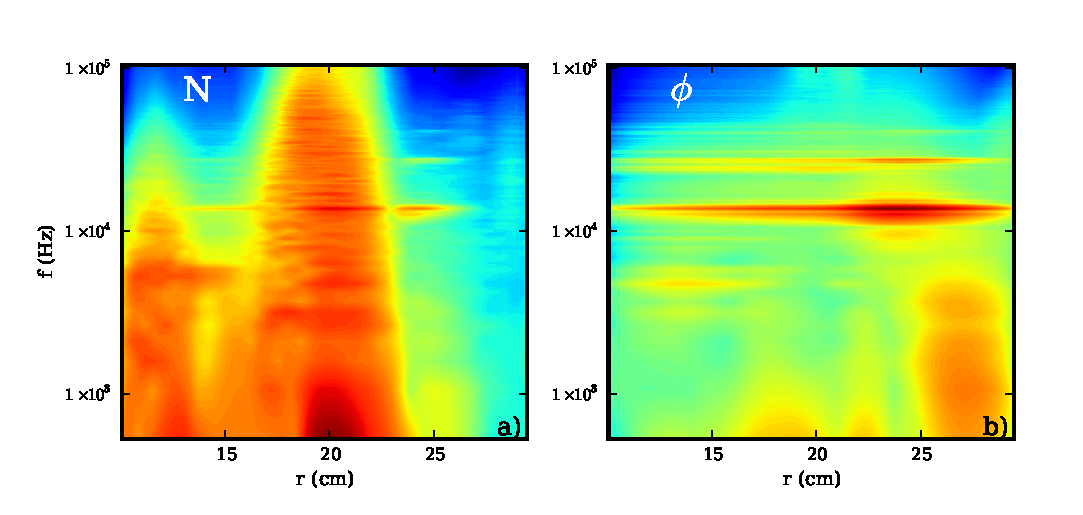
\includegraphics[]{coherent_r_f_spec}}
\caption{Radial frequency power spectra for the high flow simulation}
\label{coherent_r_f_spec}
\end{figure}

In Sec.~\ref{s_biasing_exp}, I mentioned that Schaffner et al.~\cite{schaffner2012} identified a coherent mode that grows within the broadband turbulence when the mean 
flow becomes large due to high biasing. 
In fact, I reproduce in the simulation a signature of the coherent mode, namely the peak at about $12$ kHz in the frequency spectrum (Fig.~\ref{flow_statistics} g)).
That means that the simulation data can be used to figure out the cause of this coherent mode.

In order to understand the coherent mode better, I first look at the frequency spectra as a function of radius, which I show in Fig.~\ref{coherent_r_f_spec}. Figure~\ref{coherent_r_f_spec} a)
is the spectrum of the density fluctuations, while Fig.~\ref{coherent_r_f_spec} b) is the spectrum of the potential fluctuations. The difference between the spectra of the two fields is remarkable,
with the potential having a coherent spectra and the density having a broadband spectra. While the $12$ kHz coherent mode shows up in both fields, it is far more significant in the potential field.
This indicates that the coherent mode is a flow-driven mode as opposed to a drift wave, which shouldn't be too surprising given that the mode emerges only when the flow becomes large.
Furthermore, the coherent mode is somewhat localized at a radial position around $23-26$ cm. By comparing this to Fig.~\ref{flow_profiles} f), one sees that this mode peaks where the flow shear
peaks, but where the flow magnitude is small, which provides evidence that the mode is KH-driven rather than RIC-driven. To further test this, I run two more simulations -- one removing
the KH term in Eq.~\ref{rho_eq_flow}, the other removing the RIC term. I display the radial frequency spectra of these two simulations in Fig.~\ref{coherent_r_f_spec_removals}.
The results of these simulations are not that straight-forward. When I remove the KH term, the coherent mode at $12$ kHz disappears, and the frequency spectrum of the potential changes significantly,
somewhat validating the idea that the coherent mode is KH-driven. However, removal of the RIC term also has an effect on the coherent mode. It shifts its frequency. While there is still a sharp peak
in the spectrum at about $12$ kHz, there is a more significant peak at about $7$ kHz, meaning that the $12$ kHz peak is probably just a side-band of this. Likely, the coherent mode is KH-driven,
but the RIC term shifts the frequency of the mode, though it's not obvious why it would do so.

\begin{figure}
\centerline{\includegraphics[]{coherent_r_f_spec_removals}}
\caption{Frequency power spectra without KH or RIC term}
\label{coherent_r_f_spec_removals}
\end{figure}

To further test the KH-driven coherent mode hypothesis, I look at the energy dynamics of the full simulation with both the KH and RIC terms included. However, in order to try to isolate the coherent
mode, I volume average over only the annulus in the $23-26$ cm radial domain, which should eliminate the background that is still largely controlled by the nonlinear instability. I do not show
any specific results of the energy dynamics, but qualitatively in this domain, the KH mechanism injects energy into the system, primarily at $n=0$ and at $m=1,2$. The RIC, on the other hand,
is not active here, and the nonlinear instability is also not strong here. The evidence, then, points to a KH-driven coherent mode where the RIC only affects its frequency.
